%
% $Id$
%
%%%%%%%%%%%%%%%%%%%%%%%%%%%%%%%%%%%%%%%%%%%%%%%%%%%%%%%
%
%           Copyright 2003-2007 by ACceSS MNRF
%       Copyright 2007 by University of Queensland
%
%                http://esscc.uq.edu.au
%        Primary Business: Queensland, Australia
%  Licensed under the Open Software License version 3.0
%     http://www.opensource.org/licenses/osl-3.0.php
%
%%%%%%%%%%%%%%%%%%%%%%%%%%%%%%%%%%%%%%%%%%%%%%%%%%%%%%%
%

\chapter{ The Module \finley}
 \label{CHAPTER ON FINLEY}

\begin{figure}
\centerline{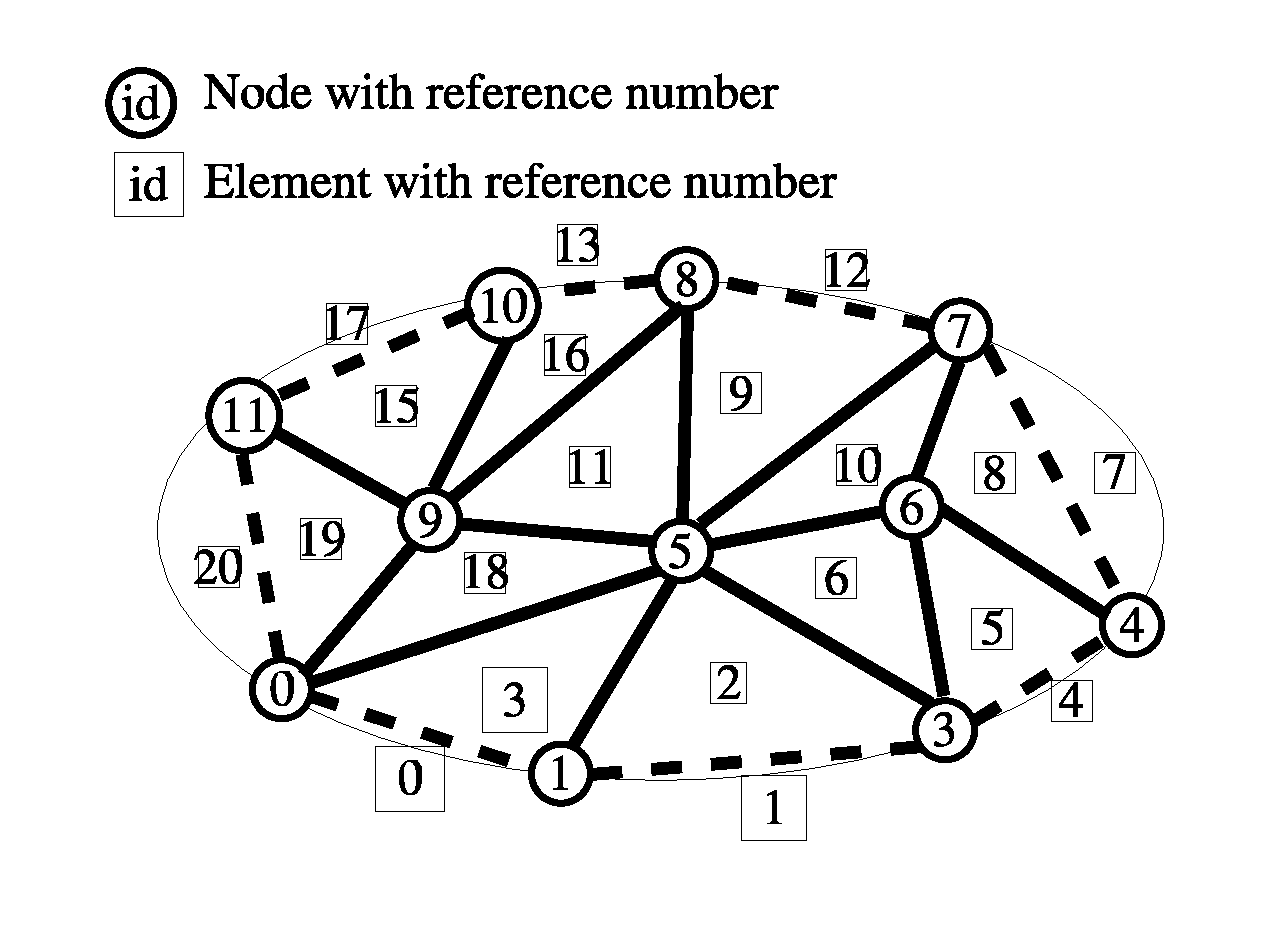
\includegraphics[width=\figwidth]{figures/FinleyMesh.eps}}
\caption{Subdivision of an Ellipse into triangles order 1 (\finleyelement{Tri3})}
\label{FINLEY FIG 0}
\end{figure}

\begin{figure}
\centerline{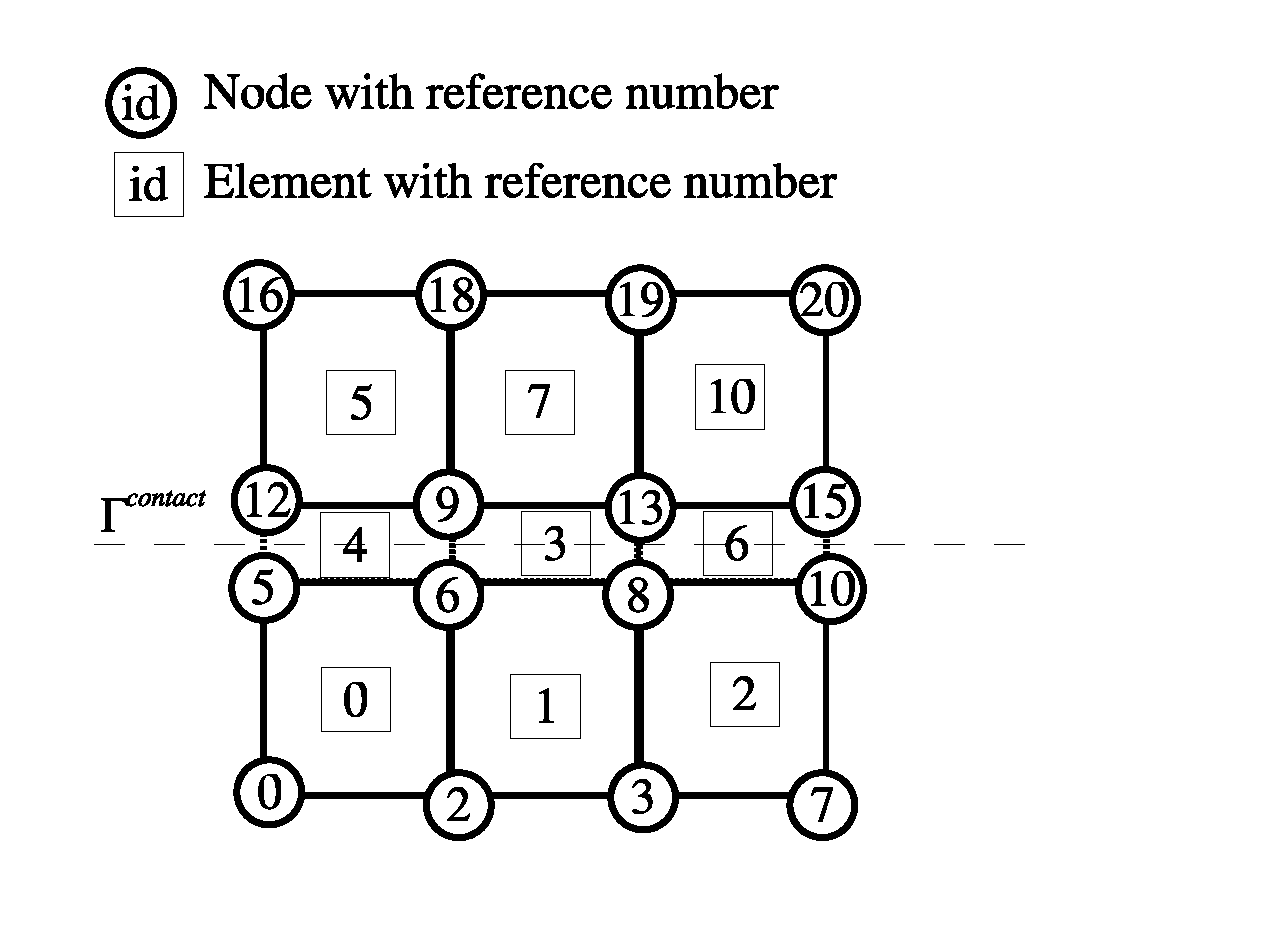
\includegraphics[width=\figwidth]{figures/FinleyContact.eps}}
\caption{Mesh around a contact region (\finleyelement{Rec4})}
\label{FINLEY FIG 01}
\end{figure}

\declaremodule{extension}{finley} \modulesynopsis{Solving linear, steady partial differential equations using
finite elements}

{\it finley} is a library of C functions solving linear, steady partial differential equations
\index{partial differential equations} (PDEs) or systems of PDEs using isoparametrical finite 
elements \index{FEM!isoparametrical}.
It supports unstructured, 1D, 2D and 3D meshes. The module \finley provides an access to the
library through the \LinearPDE class of \escript supporting its full functionality. {\it finley} 
is parallelized using the OpenMP \index{OpenMP} paradigm. 

\section{Formulation}

For a single PDE with a solution with a single component the linear PDE is defined in the
following form:
\begin{equation}\label{FINLEY.SINGLE.1}
\begin{array}{cl} &
\displaystyle{
\int\hackscore{\Omega} 
A\hackscore{jl} \cdot v\hackscore{,j}u\hackscore{,l}+ B\hackscore{j} \cdot v\hackscore{,j} u+ C\hackscore{l} \cdot v u\hackscore{,l}+D \cdot vu \; d\Omega }  \\
+ & \displaystyle{\int\hackscore{\Gamma} d \cdot vu \; d{\Gamma} } 
+  \displaystyle{\int\hackscore{\Gamma^{contact}} d^{contact} \cdot [v][u] \; d{\Gamma} } \\
= & \displaystyle{\int\hackscore{\Omega}  X\hackscore{j} \cdot v\hackscore{,j}+ Y \cdot v \; d\Omega }\\ 
+ & \displaystyle{\int\hackscore{\Gamma} y \cdot v \; d{\Gamma}}  + 
\displaystyle{\int\hackscore{\Gamma^{contact}} y^{contact}\cdot [v] \; d{\Gamma}} \\
\end{array}
\end{equation}

\section{Meshes}
To understand the usage of \finley one needs to have an understanding of how the finite element meshes
\index{FEM!mesh} are defined. \fig{FINLEY FIG 0} shows an example of the
subdivision of an ellipse into so called elements \index{FEM!elements} \index{element}. 
In this case, triangles have been used but other forms of subdivisions
can be constructed, e.g. into quadrilaterals or, in the three dimensional case, into tetrahedrons
and hexahedrons. The idea of the finite element method is to approximate the solution by a function
which is a polynomial of a certain order and is continuous across it boundary to neighbour elements.
In the example of \fig{FINLEY FIG 0} a linear polynomial is used on each triangle. As one can see, the triangulation
is quite a poor approximation of the ellipse. It can be improved by introducing a midpoint on each element edge then
positioning those nodes located on an edge expected to describe the boundary, onto the boundary.
In this case the triangle gets a curved edge which requires a parametrization of the triangle using a 
quadratic polynomial. For this case, the solution is also approximated by a piecewise quadratic polynomial
(which explains the name isoparametrical elements), see \Ref{Zienc,NumHand} for more details.   

The union of all elements defines the domain of the PDE.
Each element is defined by the nodes used to describe its shape. In \fig{FINLEY FIG 0} the element,
which has type \finleyelement{Tri3},
with element reference number $19$ \index{element!reference number} is defined by the nodes
with reference numbers $9$, $11$ and $0$ \index{node!reference number}. Notice that the order is counterclockwise. 
The coefficients of the PDE are evaluated at integration nodes with each individual element. 
For quadrilateral elements a Gauss quadrature scheme is used. In the case of triangular elements a 
modified form is applied. The boundary of the domain is also subdivided into elements. \index{element!face} In \fig{FINLEY FIG 0}
line elements with two nodes are used. The elements are also defined by their describing nodes, e.g.
the face element reference number $20$ which has type \finleyelement{Line2} is defined by the nodes
with the reference numbers $11$ and $0$. Again the order is crucial, if moving from the first
to second node the domain has to lie on the left hand side (in the case of a two dimension surface element
the domain has to lie on the left hand side when moving counterclockwise). If the gradient on the
surface of the domain is to be calculated rich face elements face to be used. Rich elements on a face
are identical to interior elements but with a modified order of nodes such that the 'first' face of the element aligns
with the surface of the domain. In \fig{FINLEY FIG 0}
elements of the type \finleyelement{Tri3Face} are used. 
The face element reference number $20$ as a rich face element is defined by the nodes
with reference numbers $11$, $0$ and $9$. Notice that the face element $20$ is identical to the
interior element $19$ except that, in this case, the order of the node is different to align the first
edge of the triangle (which is the edge starting with the first node) with the boundary of the domain.

Be aware that face elements and elements in the interior of the domain must match, i.e. a face element must be the face
of an interior element or, in case of a rich face element, it must be identical to an interior element.
If no face elements are specified
\finley implicitly assumes homogeneous natural boundary conditions \index{natural boundary conditions!homogeneous},
i.e. \var{d}=$0$ and \var{y}=$0$, on the entire boundary of the domain. For  
inhomogeneous natural boundary conditions \index{natural boundary conditions!inhomogeneous}, 
the boundary must be described by face elements. 

If discontinuities of the PDE solution are considered contact elements 
\index{element!contact}\index{contact conditions} are introduced to describe the contact region $\Gamma^{contact}$ 
even if $d^{contact}$ and $y^{contact}$ are zero. \fig{FINLEY FIG 01} shows a simple example of a mesh
of rectangular elements around a contact region $\Gamma^{contact}$ \index{element!contact}. 
The contact region is described by the
elements $4$, $3$ and $6$. Their element type is \finleyelement{Line2_Contact}. 
The nodes $9$, $12$, $6$, $5$ define contact element $4$, where the coordinates of nodes $12$ and $5$ and
nodes $4$ and $6$ are identical with the idea that nodes $12$ and $9$ are located above and 
nodes $5$ and $6$ below the contact region.  
Again, the order of the nodes within an element is crucial. There is also the option of using rich elements
if the gradient is to be calculated on the contact region. Similarly to the rich face elements 
these are constructed from two interior elements by reordering the nodes such that
the 'first' face of the element above and the 'first' face of the element below the 
contact regions line up.  The rich version of element 
$4$ is of type \finleyelement{Rec4Face_Contact} and is defined by the nodes $9$, $12$, $16$, $18$, $6$, $5$, $0$ and 
$2$.

\tab{FINLEY TAB 1} shows the interior element types and the corresponding element types to be used
on the face and contacts. \fig{FINLEY.FIG:1}, \fig{FINLEY.FIG:2} and \fig{FINLEY.FIG:4} show the ordering of
the nodes within an element.

\begin{table}
\begin{tablev}{l|llll}{textrm}{interior}{face}{rich face}{contact}{rich contact}
\linev{\finleyelement{Line2}}{\finleyelement{Point1}}{\finleyelement{Line2Face}}{\finleyelement{Point1_Contact}}{\finleyelement{Line2Face_Contact}}
\linev{\finleyelement{Line3}}{\finleyelement{Point1}}{\finleyelement{Line3Face}}{\finleyelement{Point1_Contact}}{\finleyelement{Line3Face_Contact}}
\linev{\finleyelement{Tri3}}{\finleyelement{Line2}}{\finleyelement{Tri3Face}}{\finleyelement{Line2_Contact}}{\finleyelement{Tri3Face_Contact}}
\linev{\finleyelement{Tri6}}{\finleyelement{Line3}}{\finleyelement{Tri6Face}}{\finleyelement{Line3_Contact}}{\finleyelement{Tri6Face_Contact}}
\linev{\finleyelement{Rec4}}{\finleyelement{Line2}}{\finleyelement{Rec4Face}}{\finleyelement{Line2_Contact}}{\finleyelement{Rec4Face_Contact}}
\linev{\finleyelement{Rec8}}{\finleyelement{Line3}}{\finleyelement{Rec8Face}}{\finleyelement{Line3_Contact}}{\finleyelement{Rec8Face_Contact}}
\linev{\finleyelement{Rec9}}{\finleyelement{Line3}}{\finleyelement{Rec9Face}}{\finleyelement{Line3_Contact}}{\finleyelement{Rec9Face_Contact}}
\linev{\finleyelement{Tet4}}{\finleyelement{Tri6}}{\finleyelement{Tet4Face}}{\finleyelement{Tri6_Contact}}{\finleyelement{Tet4Face_Contact}}
\linev{\finleyelement{Tet10}}{\finleyelement{Tri9}}{\finleyelement{Tet10Face}}{\finleyelement{Tri9_Contact}}{\finleyelement{Tet10Face_Contact}}
\linev{\finleyelement{Hex8}}{\finleyelement{Rec4}}{\finleyelement{Hex8Face}}{\finleyelement{Rec4_Contact}}{\finleyelement{Hex8Face_Contact}}
\linev{\finleyelement{Hex20}}{\finleyelement{Rec8}}{\finleyelement{Hex20Face}}{\finleyelement{Rec8_Contact}}{\finleyelement{Hex20Face_Contact}}
\end{tablev}
\caption{Finley elements and corresponding elements to be used on domain faces and contacts.
The rich types have to be used if the gradient of function is to be calculated on faces and contacts, respectively.}
\label{FINLEY TAB 1}
\end{table}

The native \finley file format is defined as follows.
Each node \var{i} has \var{dim} spatial coordinates \var{Node[i]}, a reference number
\var{Node_ref[i]}, a degree of freedom \var{Node_DOF[i]} and tag \var{Node_tag[i]}.
In most cases \var{Node_DOF[i]}=\var{Node_ref[i]} however, for periodic boundary conditions,
\var{Node_DOF[i]} is chosen differently, see example below. The tag can be used to mark nodes sharing
the same properties. Element \var{i} is defined by the \var{Element_numNodes} nodes \var{Element_Nodes[i]}
which is a list of node reference numbers. The order is crucial.
It has a reference number \var{Element_ref[i]} and a tag \var{Element_tag[i]}. The tag 
can be used to mark elements  sharing the same properties. For instance elements above 
a contact region are marked with $2$ and elements below a contact region are marked with $1$. 
\var{Element_Type} and \var{Element_Num} give the element type and the number of elements in the mesh.
Analogue notations are used for face and contact elements. The following Python script
prints the mesh definition in the \finley file format:
\begin{python}
print "%s\n"%mesh_name
# node coordinates:
print "%dD-nodes %d\n"%(dim,numNodes)
for i in range(numNodes): 
   print "%d %d %d"%(Node_ref[i],Node_DOF[i],Node_tag[i])
   for j in range(dim): print " %e"%Node[i][j]
   print "\n"
# interior elements
print "%s %d\n"%(Element_Type,Element_Num)
for i in range(Element_Num):
   print "%d %d"%(Element_ref[i],Element_tag[i])
   for j in range(Element_numNodes): print " %d"%Element_Nodes[i][j]
   print "\n"
# face elements
print "%s %d\n"%(FaceElement_Type,FaceElement_Num)
for i in range(FaceElement_Num):
   print "%d %d"%(FaceElement_ref[i],FaceElement_tag[i])
   for j in range(FaceElement_numNodes): print " %d"%FaceElement_Nodes[i][j]
   print "\n"
# contact elements
print "%s %d\n"%(ContactElement_Type,ContactElement_Num)
for i in range(ContactElement_Num):
   print "%d %d"%(ContactElement_ref[i],ContactElement_tag[i])
   for j in range(ContactElement_numNodes): print " %d"%ContactElement_Nodes[i][j]
   print "\n"
# point sources (not supported yet)
write("Point1 0",face_element_type,numFaceElements)
\end{python}

The following example of a mesh file defines the mesh shown in \fig{FINLEY FIG 01}:
\begin{verbatim}
Example 1
2D Nodes 16
0   0 0 0.   0.
2   2 0 0.33 0.
3   3 0 0.66 0.
7   4 0 1.   0.
5   5 0 0.   0.5
6   6 0 0.33 0.5
8   8 0 0.66 0.5
10 10 0 1.0  0.5
12 12 0 0.   0.5
9   9 0 0.33 0.5
13 13 0 0.66 0.5
15 15 0 1.0  0.5
16 16 0 0.   1.0
18 18 0 0.33 1.0
19 19 0 0.66 1.0
20 20 0 1.0  1.0
Rec4 6
 0 1  0  2  6  5
 1 1  2  3  8  6
 2 1  3  7 10  8
 5 2 12  9 18 16
 7 2 13 19 18  9
10 2 20 19 13 15
Line2 0
Line2_Contact 3
 4 0  9 12  6 5
 3 0 13  9  8 6
 6 0 15 13 10 8
Point1 0
\end{verbatim}
Notice that the order in which the nodes and elements are given is arbitrary.
In the case that rich contact elements are used the contact element section gets
 the form
\begin{verbatim}
Rec4Face_Contact 3
 4 0  9 12 16 18  6  5  0  2
 3 0 13  9 18 19  8  6  2  3
 6 0 15 13 19 20 10  8  3  7
\end{verbatim}
Periodic boundary condition \index{boundary conditions!periodic} can be introduced by altering \var{Node_DOF}.
It allows identification of nodes even if they have different physical locations. For instance, to
enforce periodic boundary conditions at the face $x_0=0$ and $x_0=1$ one identifies
the degrees of freedom for nodes $0$, $5$, $12$ and $16$ with the degrees of freedom for
$7$, $10$, $15$ and $20$, respectively. The node section of the \finley mesh gets now the form:  
\begin{verbatim}
2D Nodes 16
0   0 0 0.   0.
2   2 0 0.33 0.
3   3 0 0.66 0.
7   0 0 1.   0.
5   5 0 0.   0.5
6   6 0 0.33 0.5
8   8 0 0.66 0.5
10  5 0 1.0  0.5
12 12 0 0.   0.5
9   9 0 0.33 0.5
13 13 0 0.66 0.5
15 12 0 1.0  0.5
16 16 0 0.   1.0
18 18 0 0.33 1.0
19 19 0 0.66 1.0
20 16 0 1.0  1.0
\end{verbatim}



%%%%%%%%%%%%%%%%%%%%%%%%%%%%%%%%%%%%%%%%%%%%%%%%%%%%%%%%%%%%%%%%%%%%%%%%%%%%%%
% Copyright (c) 2003-2015 by University of Queensland
% http://www.uq.edu.au
%
% Primary Business: Queensland, Australia
% Licensed under the Open Software License version 3.0
% http://www.opensource.org/licenses/osl-3.0.php
%
% Development until 2012 by Earth Systems Science Computational Center (ESSCC)
% Development 2012-2013 by School of Earth Sciences
% Development from 2014 by Centre for Geoscience Computing (GeoComp)
%
%%%%%%%%%%%%%%%%%%%%%%%%%%%%%%%%%%%%%%%%%%%%%%%%%%%%%%%%%%%%%%%%%%%%%%%%%%%%%%

\setlength{\unitlength}{1mm}

\newsavebox{\HLa}
\savebox{\HLa}(0,0)
  {\put(0,0){\circle*{2}}
   \thicklines \put(1,0){\line(1,0){28}}
   \put(30,0){\circle*{2}} }

\newsavebox{\HLathin}
\savebox{\HLathin}(0,0)
  {\put(0,0){\circle{2}}
   \thinlines \put(1,0){\line(1,0){28}}
   \put(30,0){\circle{2}} }

\newsavebox{\VLa}
\savebox{\VLa}(0,30)
  {\put(0,0){\circle*{2}}
   \thicklines \put(0,1){\line(0,1){28}}
   \put(0,30){\circle*{2}} }

\newsavebox{\VLathin}
\savebox{\VLathin}(0,30)
  {\put(0,0){\circle{2}}
   \thinlines \put(0,1){\line(0,1){28}}
   \put(0,30){\circle{2}} }

\newsavebox{\SLax}
\savebox{\SLax}(0,30)
  {\thicklines \put(0,0){\line(-1,1){30}}
   \put(0,0){\circle*{2}}
   \put(-30,30){\circle*{2}} }

\newsavebox{\SLaa}
\savebox{\SLaa}(0,15)
  {\thicklines \put(0,0){\line(-4,3){20}}
   \put(0,0){\circle*{2}}
   \put(-20,15){\circle*{2}} }

\newsavebox{\SLab}
\savebox{\SLab}(0,-15)
  {\thicklines \put(0,0){\line(-4,-3){20}}
   \put(0,0){\circle*{2}}
   \put(-20,-15){\circle*{2}} }

\newsavebox{\SLabthin}
\savebox{\SLabthin}(0,-15)
  {\thinlines \put(-0.7,-0.7){\line(-4,-3){18.7}}
   \put(0,0){\circle{2}}
   \put(-20,-15){\circle{2}} }

\newsavebox{\SLac}
\savebox{\SLac}(0,15)
  {\thicklines \put(0,0){\line(-2,3){10}}
   \put(0,0){\circle*{2}}
   \put(-10,15){\circle*{2}} }

\newsavebox{\SLacthin}
\savebox{\SLacthin}(0,15)
  {\thinlines \put(0,0){\line(-2,3){9.4}}
   \put(0,0){\circle{2}}
   \put(-10,15){\circle{2}} }


\newsavebox{\HLd}
\savebox{\HLd}(0,0)
  {\put(0,0){\circle*{2}}
   \put(10,0){\circle*{2}}
   \thicklines \put(1,0){\line(1,0){28}}
   \put(20,0){\circle*{2}}
   \put(30,0){\circle*{2}} }

\newsavebox{\HLdthin}
\savebox{\HLdthin}(0,0)
  {\put(0,0){\circle{2}}
   \put(10,0){\circle{2}}
   \thinlines \multiput(1,0)(10,0){3}{\line(1,0){8}}
   \put(20,0){\circle{2}}
   \put(30,0){\circle{2}} }

\newsavebox{\VLd}
\savebox{\VLd}(0,30)
  {\put(0,0){\circle*{2}}
   \put(0,10){\circle*{2}}
   \thicklines \put(0,1){\line(0,1){28}}
   \put(0,20){\circle*{2}}
   \put(0,30){\circle*{2}} }

\newsavebox{\VLdthin}
\savebox{\VLdthin}(0,30)
  {\put(0,0){\circle{2}}
   \put(0,10){\circle{2}}
   \thinlines \multiput(0,1)(0,10){3}{\line(0,1){8}}
   \put(0,20){\circle{2}}
   \put(0,30){\circle{2}} }

\newsavebox{\SLf}
\savebox{\SLf}(0,30)
  {\thicklines \put(0,0){\line(-1,1){30}}
   \put(0,0){\circle*{2}}
   \put(-10,10){\circle*{2}}
   \put(-20,20){\circle*{2}}
   \put(-30,30){\circle*{2}} }

\newsavebox{\SLad}
\savebox{\SLad}(0,15)
  {\thicklines \put(0,0){\line(-4,3){20}}
   \put(0,0){\circle*{2}}
   \put(-6.66,5){\circle*{2}}
   \put(-13.33,10){\circle*{2}}
   \put(-20,15){\circle*{2}} }

\newsavebox{\SLbd}
\savebox{\SLbd}(0,-15)
  {\thicklines \put(0,0){\line(-4,-3){20}}
   \put(0,0){\circle*{2}}
   \put(-6.66,-5){\circle*{2}}
   \put(-13.33,-10){\circle*{2}}
   \put(-20,-15){\circle*{2}} }

\newsavebox{\SLbdthin}
\savebox{\SLbdthin}(0,-15)
  {\thinlines \multiput(-0.7,-0.7)(-6.66,-5){3}{\line(-4,-3){5.1}}
   \put(0,0){\circle{2}}
   \put(-6.66,-5){\circle{2}}
   \put(-13.33,-10){\circle{2}}
   \put(-20,-15){\circle{2}} }

\newsavebox{\SLcd}
\savebox{\SLcd}(0,15)
  {\thicklines \put(0,0){\line(-2,3){10}}
   \put(0,0){\circle*{2}}
   \put(-3.33,5){\circle*{2}}
   \put(-6.66,10){\circle*{2}}
   \put(-10,15){\circle*{2}} }

\newsavebox{\SLcdthin}
\savebox{\SLcdthin}(0,15)
  {\thinlines \multiput(-0.6,0.8)(-3.33,5){3}{\line(-2,3){2.35}}
   \put(0,0){\circle{2}}
   \put(-3.33,5){\circle{2}}
   \put(-6.66,10){\circle{2}}
   \put(-10,15){\circle{2}} }

\newsavebox{\HLe}
\savebox{\HLe}(0,0)
  {\put(0,0){\circle*{2}}
   \put(15,0){\circle*{2}}
   \thicklines \put(1,0){\line(1,0){28}}
   \put(30,0){\circle*{2}} }

\newsavebox{\HLethin}
\savebox{\HLethin}(0,0)
  {\put(0,0){\circle{2}}
   \put(15,0){\circle{2}}
   \thinlines \multiput(1,0)(15,0){2}{\line(1,0){13}}
   \put(30,0){\circle{2}} }

\newsavebox{\VLe}
\savebox{\VLe}(0,30)
  {\put(0,0){\circle*{2}}
   \put(0,15){\circle*{2}}
   \thicklines \put(0,1){\line(0,1){28}}
   \put(0,30){\circle*{2}} }

\newsavebox{\VLethin}
\savebox{\VLethin}(0,30)
  {\put(0,0){\circle{2}}
   \put(0,15){\circle{2}}
   \thinlines \multiput(0,1)(0,15){2}{\line(0,1){13}}
   \put(0,30){\circle{2}} }

\newsavebox{\SLe}
\savebox{\SLe}(0,30)
  {\thicklines \put(0,0){\line(-1,1){30}}
   \put(0,0){\circle*{2}}
   \put(-15,15){\circle*{2}}
   \put(-30,30){\circle*{2}} }

\newsavebox{\SLae}
\savebox{\SLae}(0,15)
  {\thicklines \put(0,0){\line(-4,3){20}}
   \put(0,0){\circle*{2}}
   \put(-10,7.5){\circle*{2}}
   \put(-20,15){\circle*{2}} }

\newsavebox{\SLbe}
\savebox{\SLbe}(0,-15)
  {\thicklines \put(0,0){\line(-4,-3){20}}
   \put(0,0){\circle*{2}}
   \put(-10,-7.5){\circle*{2}}
   \put(-20,-15){\circle*{2}} }

\newsavebox{\SLbethin}
\savebox{\SLbethin}(0,-15)
  {\thinlines \multiput(-0.7,-0.7)(-10,-7.5){2}{\line(-4,-3){8.4}}
   \put(0,0){\circle{2}}
   \put(-10,-7.5){\circle{2}}
   \put(-20,-15){\circle{2}} }

\newsavebox{\SLce}
\savebox{\SLce}(0,15)
  {\thicklines \put(0,0){\line(-2,3){10}}
   \put(0,0){\circle*{2}}
   \put(-5,7.5){\circle*{2}}
   \put(-10,15){\circle*{2}} }

\newsavebox{\SLcethin}
\savebox{\SLcethin}(0,15)
  {\thinlines \multiput(-0.6,0.8)(-5,7.5){2}{\line(-2,3){3.9}}
   \put(0,0){\circle{2}}
   \put(-5,7.5){\circle{2}}
   \put(-10,15){\circle{2}} }

%=====================================================================
%
%   order 1
%   -------
%

\begin{figure}
\begin{center}
\begin{picture}(150,160) \thicklines

\put(20,155){\circle*{2}}
\put(15,145){\parbox[t]{45mm}
             \finleyelement{Point1}}

\put(90,155){\usebox{\HLa}}
\put(90,145){\parbox[t]{45mm}
             \finleyelement{Line2} }

\put(10,95){\usebox{\HLa}}
\put(40,95){\usebox{\SLax}}
\put(10,95){\usebox{\VLa}}
\put(10,85){\parbox[t]{45mm}
             \finleyelement{Tri3} }

\put(90,95){\usebox{\HLa}}
\put(90,125){\usebox{\HLa}}
\put(90,95){\usebox{\VLa}}
\put(120,95){\usebox{\VLa}}
\put(90,85){\parbox[t]{45mm}
             \finleyelement{Rec4} }

\put(10,20){\usebox{\HLa}}
\put(40,20){\usebox{\SLax}}
\put(10,20){\usebox{\VLa}}
\put(40,20){\usebox{\SLac}}
\put(30,35){\usebox{\SLabthin}}
\put(30,35){\usebox{\SLaa}}
\put(10,10 ){\parbox[t]{45mm}
             \finleyelement{Tet4} }

\put(90,20){\usebox{\HLa}}
\put(90,50){\usebox{\HLa}}
\put(90,20){\usebox{\VLa}}
\put(120,20){\usebox{\VLa}}
\put(110,35){\usebox{\SLabthin}}
\put(140,35){\usebox{\SLab}}
\put(110,65){\usebox{\SLab}}
\put(140,65){\usebox{\SLab}}
\put(110,35){\usebox{\HLathin}}
\put(110,65){\usebox{\HLa}}
\put(110,35){\usebox{\VLathin}}
\put(140,35){\usebox{\VLa}}
\put(90,10 ){\parbox[t]{45mm}
             \finleyelement{Hex8} }

% numbering the lines:
 % Point
\put(19,158){{\it 1}}
% line
\put(89,158){{\it 1}} 
\put(119,158){{\it 2}}
% Triangle
\put(6,124){{\it 3}}
\put(6,94){{\it 1}}
\put(43,94){{\it 2}}
% quadrilateral
\put(86,124){{\it 4}}
\put(86,94){{\it 1}}
\put(123,124){{\it 3}}
\put(123,94){{\it 2}}
% Tetrahedron
\put(6,49){{\it 4}}
\put(6,19){{\it 1}}
\put(43,19){{\it 2}}
\put(33,34){{\it 3}}
% Hexahedron
\put(86,49){{\it 5}} 
\put(86,19){{\it 1}}
\put(123,49){{\it 6}}
\put(123,19){{\it 2}}
\put(106,64){{\it 8}}
\put(106,34){{\it 4}}
\put(143,64){{\it 7}}
\put(143,34){{\it 3}}
\end{picture}
\caption{\label{FINLEY.FIG:1} Elements of order 1}
\end{center}
\end{figure}
%=====================================================================
%
%
%   order 2
%   -------
%   (boxes in 'fesubelm')


\begin{figure}
\begin{center}
\setlength{\unitlength}{1mm}
\begin{picture}(150,160) \thicklines

\put(20,155){\circle*{2}}
\put(15,145){\parbox[t]{45mm}
             \finleyelement{Point1} }

\put(90,155){\usebox{\HLe}}
\put(90,145){\parbox[t]{45mm}
             \finleyelement{Line3} and \finleyelement{Line3Macro} }

\put(10,95){\usebox{\HLe}}
\put(40,95){\usebox{\SLe}}
\put(10,95){\usebox{\VLe}}
\put(10,85){\parbox[t]{45mm}
             \finleyelement{Tri6} }

\put(90,95){\usebox{\HLe}}
\put(90,125){\usebox{\HLe}}
\put(90,95){\usebox{\VLe}}
\put(120,95){\usebox{\VLe}}
\put(90,85){\parbox[t]{45mm}
             \finleyelement{Rec8} }

\put(10,20){\usebox{\HLe}}
\put(40,20){\usebox{\SLe}}
\put(10,20){\usebox{\VLe}}
\put(40,20){\usebox{\SLce}}
\put(30,35){\usebox{\SLbethin}}
\put(30,35){\usebox{\SLae}}
\put(10,10 ){\parbox[t]{45mm}
             \finleyelement{Tet10} and \finleyelement{Tet10Macro}}

\put(90,20){\usebox{\HLe}}
\put(90,50){\usebox{\HLe}}
\put(90,20){\usebox{\VLe}}
\put(120,20){\usebox{\VLe}}
\put(110,35){\usebox{\SLbethin}}
\put(140,35){\usebox{\SLbe}}
\put(110,65){\usebox{\SLbe}}
\put(140,65){\usebox{\SLbe}}
\put(110,35){\usebox{\HLethin}}
\put(110,65){\usebox{\HLe}}
\put(110,35){\usebox{\VLethin}}
\put(140,35){\usebox{\VLe}}
\put(90,10 ){\parbox[t]{45mm}
             \finleyelement{Hex20} }


% numbering the lines:
% Point
\put(19,158){{\it 1}} 
% line
\put(89,158){{\it 1}} 
\put(104,158){{\it 3}}
\put(119,158){{\it 2}}
% Triangle
\put(6,124){{\it 3}} 
\put(6,109){{\it 6}}
\put(6,94){{\it 1}}
\put(28,109){{\it 5}}
\put(43,94){{\it 2}}
\put(24,90){{\it 4}}
% quaTrilateral
\put(104,90){{\it 5}} 
\put(86,124){{\it 4}}
\put(86,109){{\it 8}}
\put(86,94){{\it 1}}
\put(104,128){{\it 7}}
\put(123,124){{\it 3}}
\put(123,109){{\it 6}}
\put(123,94){{\it 2}}
% Tetrahedron
\put(24,15){{\it 5}} 
\put(6,49){{\it 4}}
\put(6,34){{\it 8}}
\put(6,19){{\it 1}}
\put(21,34){{\it 9}}
\put(43,19){{\it 2}}
\put(16,26.5){{\it 7}}
\put(38,26.5){{\it 6}}
\put(33,34){{\it 3}}
\put(22.5,41.5){{\it 10}}
% Hexahedron
\put(104,15){{\it 9}} 
\put(86,49){{\it 5}}
\put(85,34){{\it 13}}
\put(86,19){{\it 1}}
\put(104,52){{\it 17}}
\put(123,49){{\it 6}}
\put(115,37){{\it 14}}
\put(123,19){{\it 2}}
\put(125,37){{\it 11}}
\put(106,64){{\it 8}}
\put(112,46){{\it 16}}
\put(106,34){{\it 4}}
\put(124,68){{\it 19}}
\put(143,64){{\it 7}}
\put(142,49){{\it 15}}
\put(143,34){{\it 3}}
\put(94.5,26.5){{\it 12}}
\put(132.5,26.5){{\it 10}}
\put(94.5,56.5){{\it 20}}
\put(132.5,56.5){{\it 18}}

\end{picture}
\caption{\label{FINLEY.FIG:2} Elements of order 2 and macro elements}
\end{center}
\end{figure}

%
% additional elements
%
\begin{figure}
\begin{center}
\begin{picture}(50,50) \thicklines
\put(10,10){\usebox{\HLe}}
\put(10,40){\usebox{\HLe}}
\put(10,10){\usebox{\VLe}}
\put(40,10){\usebox{\VLe}}
\put(25,25){\circle*{2}}
% \put(50,085){\parbox[t]{45mm}
%              \finleyelement{Rec9} and  \finleyelement{Rec9Macro}}
\put(24,5){{\it 5}}
\put(6,39){{\it 4}}
\put(6,24){{\it 8}}
\put(6,9){{\it 1}}
\put(24,43){{\it 7}}
\put(43,43){{\it 3}}
\put(43,25){{\it 6}}
\put(43,9){{\it 2}}
\put(24,20){{\it 9}}
\end{picture}
\caption{\label{FINLEY.FIG:4}\finleyelement{Rec9} and  \finleyelement{Rec9Macro}}
\end{center}
\end{figure}


\subsection{Linear Solvers in \LinearPDE}
Currently \finley supports the linear solvers \PCG, \GMRES, \PRESTWENTY and \BiCGStab. 
For \GMRES the options \var{truncation} and \var{restart} of the \method{getSolution} can be
used to control the truncation and restart during iteration. Default values are
\var{truncation}=5 and \var{restart}=20.
The default solver is \BiCGStab  but if the symmetry flag is set \PCG is the default solver.
\finley supports the solver options \var{iter_max} which specifies the maximum number of iterations steps,
\var{verbose}=\True or \False and \var{preconditioner}=\constant{JACOBI} or \constant {ILU0}.
In some installations \finley supports the \Direct solver and the
solver options \var{reordering}=\constant{util.NO_REORDERING}, 
\constant{util.MINIMUM_FILL_IN} or \constant{util.NESTED_DISSECTION} (default is \constant{util.NO_REORDERING}),
\var{drop_tolerance} specifying the threshold for values to be dropped in the 
incomplete elimination process (default is 0.01) and \var{drop_storage} specifying the maximum increase 
in storage allowed in the 
incomplete elimination process (default is 1.20).

\subsection{Functions}
\begin{funcdesc}{Mesh}{fileName,integrationOrder=-1}
creates a \Domain object form the FEM mesh defined in 
file \var{fileName}. The file must be given the \finley file format.
If \var{integrationOrder} is positive, a numerical integration scheme
chosen which is accurate on each element up to a polynomial of
degree \var{integrationOrder} \index{integration order}. Otherwise
an appropriate integration order is chosen independently.
\end{funcdesc}

\begin{funcdesc}{Rectangle}{n0,n1,order=1,l0=1.,l1=1., integrationOrder=-1, \\
  periodic0=\False,periodic1=\False,useElementsOnFace=\False,optimize=\False}
Generates a \Domain object representing a two dimensional rectangle between
$(0,0)$ and $(l0,l1)$ with orthogonal edges. The rectangle is filled with
\var{n0} elements along the $x_0$-axis and
\var{n1} elements along the $x_1$-axis. 
For \var{order}=1 and \var{order}=2
\finleyelement{Rec4} and  
\finleyelement{Rec8} are used, respectively. 
In the case of \var{useElementsOnFace}=\False,
\finleyelement{Line2} and  
\finleyelement{Line3} are used to subdivide the edges of the rectangle, respectively. 
In the case of \var{useElementsOnFace}=\True (this option should be used if gradients
are calculated on domain faces),
\finleyelement{Rec4Face} and  
\finleyelement{Rec8Face} are used on the edges, respectively.  
If \var{integrationOrder} is positive, a numerical integration scheme
chosen which is accurate on each element up to a polynomial of
degree \var{integrationOrder} \index{integration order}. Otherwise
an appropriate integration order is chosen independently. If
\var{periodic0}=\True, periodic boundary conditions \index{periodic boundary conditions}
along the $x_0$-directions are enforced. That means when for any solution of a PDE solved by \finley
the value on the line $x_0=0$ will be identical to the values on $x_0=\var{l0}$.
Correspondingly,
\var{periodic1}=\False sets periodic boundary conditions
in $x_1$-direction.
If \var{optimize}=\True mesh node relabeling will be attempted to reduce the computation and also ParMETIS will be used to improve the mesh partition if running on multiple CPUs with MPI.
\end{funcdesc}

\begin{funcdesc}{Brick}{n0,n1,n2,order=1,l0=1.,l1=1.,l2=1., integrationOrder=-1, \\
  periodic0=\False,periodic1=\False,periodic2=\False,useElementsOnFace=\False,optimize=\False}
Generates a \Domain object representing a three dimensional brick between
$(0,0,0)$ and $(l0,l1,l2)$ with orthogonal faces. The brick is filled with
\var{n0} elements along the $x_0$-axis, 
\var{n1} elements along the $x_1$-axis and 
\var{n2} elements along the $x_2$-axis. 
For \var{order}=1 and \var{order}=2
\finleyelement{Hex8} and  
\finleyelement{Hex20} are used, respectively. 
In the case of \var{useElementsOnFace}=\False,
\finleyelement{Rec4} and  
\finleyelement{Rec8} are used to subdivide the faces of the brick, respectively. 
In the case of \var{useElementsOnFace}=\True (this option should be used if gradients
are calculated on domain faces),
\finleyelement{Hex8Face} and  
\finleyelement{Hex20Face} are used on the brick faces, respectively.  
If \var{integrationOrder} is positive, a numerical integration scheme
chosen which is accurate on each element up to a polynomial of
degree \var{integrationOrder} \index{integration order}. Otherwise
an appropriate integration order is chosen independently. If
\var{periodic0}=\True, periodic boundary conditions \index{periodic boundary conditions}
along the $x_0$-directions are enforced. That means when for any solution of a PDE solved by \finley
the value on the plane $x_0=0$ will be identical to the values on $x_0=\var{l0}$. Correspondingly,
\var{periodic1}=\False and \var{periodic2}=\False sets periodic boundary conditions
in $x_1$-direction and $x_2$-direction, respectively.
If \var{optimize}=\True mesh node relabeling will be attempted to reduce the computation and also ParMETIS will be used to improve the mesh partition if running on multiple CPUs with MPI.
\end{funcdesc}

\begin{funcdesc}{GlueFaces}{meshList,safetyFactor=0.2,tolerance=1.e-13}
Generates a new \Domain object from the list \var{meshList} of \finley meshes.
Nodes in face elements whose difference of coordinates is less then \var{tolerance} times the 
diameter of the domain are merged. The corresponding face elements are removed from the mesh.  

TODO: explain \var{safetyFactor} and show an example.
\end{funcdesc}

\begin{funcdesc}{JoinFaces}{meshList,safetyFactor=0.2,tolerance=1.e-13}
Generates a new \Domain object from the list \var{meshList} of \finley meshes.
Face elements whose nodes coordinates have difference is less then \var{tolerance} times the 
diameter of the domain are combined to form a contact element \index{element!contact} 
The corresponding face elements are removed from the mesh.  

TODO: explain \var{safetyFactor} and show an example.
\end{funcdesc}
